%% bare_conf.tex
%% V1.3
%% 2007/01/11
%% by Michael Shell
%% See:
%% http://www.michaelshell.org/
%% for current contact information.
%%
%% This is a skeleton file demonstrating the use of IEEEtran.cls
%% (requires IEEEtran.cls version 1.7 or later) with an IEEE conference paper.
%%
%% Support sites:
%% http://www.michaelshell.org/tex/ieeetran/
%% http://www.ctan.org/tex-archive/macros/latex/contrib/IEEEtran/
%% and
%% http://www.ieee.org/

%%*************************************************************************
%% Legal Notice:
%% This code is offered as-is without any warranty either expressed or
%% implied; without even the implied warranty of MERCHANTABILITY or
%% FITNESS FOR A PARTICULAR PURPOSE! 
%% User assumes all risk.
%% In no event shall IEEE or any contributor to this code be liable for
%% any damages or losses, including, but not limited to, incidental,
%% consequential, or any other damages, resulting from the use or misuse
%% of any information contained here.
%%
%% All comments are the opinions of their respective authors and are not
%% necessarily endorsed by the IEEE.
%%
%% This work is distributed under the LaTeX Project Public License (LPPL)
%% ( http://www.latex-project.org/ ) version 1.3, and may be freely used,
%% distributed and modified. A copy of the LPPL, version 1.3, is included
%% in the base LaTeX documentation of all distributions of LaTeX released
%% 2003/12/01 or later.
%% Retain all contribution notices and credits.
%% ** Modified files should be clearly indicated as such, including  **
%% ** renaming them and changing author support contact information. **
%%
%% File list of work: IEEEtran.cls, IEEEtran_HOWTO.pdf, bare_adv.tex,
%%                    bare_conf.tex, bare_jrnl.tex, bare_jrnl_compsoc.tex
%%*************************************************************************

% *** Authors should verify (and, if needed, correct) their LaTeX system  ***
% *** with the testflow diagnostic prior to trusting their LaTeX platform ***
% *** with production work. IEEE's font choices can trigger bugs that do  ***
% *** not appear when using other class files.                            ***
% The testflow support page is at:
% http://www.michaelshell.org/tex/testflow/



% Note that the a4paper option is mainly intended so that authors in
% countries using A4 can easily print to A4 and see how their papers will
% look in print - the typesetting of the document will not typically be
% affected with changes in paper size (but the bottom and side margins will).
% Use the testflow package mentioned above to verify correct handling of
% both paper sizes by the user's LaTeX system.
%
% Also note that the "draftcls" or "draftclsnofoot", not "draft", option
% should be used if it is desired that the figures are to be displayed in
% draft mode.
%
\documentclass[letterpaper]{IEEEtran}
% Add the compsoc option for Computer Society conferences.
%
% If IEEEtran.cls has not been installed into the LaTeX system files,
% manually specify the path to it like:
% \documentclass[conference]{../sty/IEEEtran}


\usepackage{tikz,pgf,import}
\usetikzlibrary{shapes.geometric, arrows,positioning,matrix,calc,intersections,backgrounds}
\usepackage{amsmath,caption,subcaption}
\usepackage{booktabs, multicol,multirow, makecell, afterpage}
\usepackage{tabularx, adjustbox}



% Some very useful LaTeX packages include:
% (uncomment the ones you want to load)




% *** CITATION PACKAGES ***
%
%\usepackage{cite}
% cite.sty was written by Donald Arseneau
% V1.6 and later of IEEEtran pre-defines the format of the cite.sty package
% \cite{} output to follow that of IEEE. Loading the cite package will
% result in citation numbers being automatically sorted and properly
% "compressed/ranged". e.g., [1], [9], [2], [7], [5], [6] without using
% cite.sty will become [1], [2], [5]--[7], [9] using cite.sty. cite.sty's
% \cite will automatically add leading space, if needed. Use cite.sty's
% noadjust option (cite.sty V3.8 and later) if you want to turn this off.
% cite.sty is already installed on most LaTeX systems. Be sure and use
% version 4.0 (2003-05-27) and later if using hyperref.sty. cite.sty does
% not currently provide for hyperlinked citations.
% The latest version can be obtained at:
% http://www.ctan.org/tex-archive/macros/latex/contrib/cite/
% The documentation is contained in the cite.sty file itself.


% *** MATH PACKAGES ***
%
%\usepackage[cmex10]{amsmath}
% A popular package from the American Mathematical Society that provides
% many useful and powerful commands for dealing with mathematics. If using
% it, be sure to load this package with the cmex10 option to ensure that
% only type 1 fonts will utilized at all point sizes. Without this option,
% it is possible that some math symbols, particularly those within
% footnotes, will be rendered in bitmap form which will result in a
% document that can not be IEEE Xplore compliant!
%
% Also, note that the amsmath package sets \interdisplaylinepenalty to 10000
% thus preventing page breaks from occurring within multiline equations. Use:
%\interdisplaylinepenalty=2500
% after loading amsmath to restore such page breaks as IEEEtran.cls normally
% does. amsmath.sty is already installed on most LaTeX systems. The latest
% version and documentation can be obtained at:
% http://www.ctan.org/tex-archive/macros/latex/required/amslatex/math/





% *** SPECIALIZED LIST PACKAGES ***
%
%\usepackage{algorithmic}
% algorithmic.sty was written by Peter Williams and Rogerio Brito.
% This package provides an algorithmic environment fo describing algorithms.
% You can use the algorithmic environment in-text or within a figure
% environment to provide for a floating algorithm. Do NOT use the algorithm
% floating environment provided by algorithm.sty (by the same authors) or
% algorithm2e.sty (by Christophe Fiorio) as IEEE does not use dedicated
% algorithm float types and packages that provide these will not provide
% correct IEEE style captions. The latest version and documentation of
% algorithmic.sty can be obtained at:
% http://www.ctan.org/tex-archive/macros/latex/contrib/algorithms/
% There is also a support site at:
% http://algorithms.berlios.de/index.html
% Also of interest may be the (relatively newer and more customizable)
% algorithmicx.sty package by Szasz Janos:
% http://www.ctan.org/tex-archive/macros/latex/contrib/algorithmicx/




% *** ALIGNMENT PACKAGES ***
%
%\usepackage{array}
% Frank Mittelbach's and David Carlisle's array.sty patches and improves
% the standard LaTeX2e array and tabular environments to provide better
% appearance and additional user controls. As the default LaTeX2e table
% generation code is lacking to the point of almost being broken with
% respect to the quality of the end results, all users are strongly
% advised to use an enhanced (at the very least that provided by array.sty)
% set of table tools. array.sty is already installed on most systems. The
% latest version and documentation can be obtained at:
% http://www.ctan.org/tex-archive/macros/latex/required/tools/


%\usepackage{mdwmath}
%\usepackage{mdwtab}
% Also highly recommended is Mark Wooding's extremely powerful MDW tools,
% especially mdwmath.sty and mdwtab.sty which are used to format equations
% and tables, respectively. The MDWtools set is already installed on most
% LaTeX systems. The lastest version and documentation is available at:
% http://www.ctan.org/tex-archive/macros/latex/contrib/mdwtools/


% IEEEtran contains the IEEEeqnarray family of commands that can be used to
% generate multiline equations as well as matrices, tables, etc., of high
% quality.


%\usepackage{eqparbox}
% Also of notable interest is Scott Pakin's eqparbox package for creating
% (automatically sized) equal width boxes - aka "natural width parboxes".
% Available at:
% http://www.ctan.org/tex-archive/macros/latex/contrib/eqparbox/





% *** SUBFIGURE PACKAGES ***
%\usepackage[tight,footnotesize]{subfigure}
% subfigure.sty was written by Steven Douglas Cochran. This package makes it
% easy to put subfigures in your figures. e.g., "Figure 1a and 1b". For IEEE
% work, it is a good idea to load it with the tight package option to reduce
% the amount of white space around the subfigures. subfigure.sty is already
% installed on most LaTeX systems. The latest version and documentation can
% be obtained at:
% http://www.ctan.org/tex-archive/obsolete/macros/latex/contrib/subfigure/
% subfigure.sty has been superceeded by subfig.sty.



%\usepackage[caption=false]{caption}
%\usepackage[font=footnotesize]{subfig}
% subfig.sty, also written by Steven Douglas Cochran, is the modern
% replacement for subfigure.sty. However, subfig.sty requires and
% automatically loads Axel Sommerfeldt's caption.sty which will override
% IEEEtran.cls handling of captions and this will result in nonIEEE style
% figure/table captions. To prevent this problem, be sure and preload
% caption.sty with its "caption=false" package option. This is will preserve
% IEEEtran.cls handing of captions. Version 1.3 (2005/06/28) and later 
% (recommended due to many improvements over 1.2) of subfig.sty supports
% the caption=false option directly:
%\usepackage[caption=false,font=footnotesize]{subfig}
%
% The latest version and documentation can be obtained at:
% http://www.ctan.org/tex-archive/macros/latex/contrib/subfig/
% The latest version and documentation of caption.sty can be obtained at:
% http://www.ctan.org/tex-archive/macros/latex/contrib/caption/




% *** FLOAT PACKAGES ***
%
%\usepackage{fixltx2e}
% fixltx2e, the successor to the earlier fix2col.sty, was written by
% Frank Mittelbach and David Carlisle. This package corrects a few problems
% in the LaTeX2e kernel, the most notable of which is that in current
% LaTeX2e releases, the ordering of single and double column floats is not
% guaranteed to be preserved. Thus, an unpatched LaTeX2e can allow a
% single column figure to be placed prior to an earlier double column
% figure. The latest version and documentation can be found at:
% http://www.ctan.org/tex-archive/macros/latex/base/



%\usepackage{stfloats}
% stfloats.sty was written by Sigitas Tolusis. This package gives LaTeX2e
% the ability to do double column floats at the bottom of the page as well
% as the top. (e.g., "\begin{figure*}[!b]" is not normally possible in
% LaTeX2e). It also provides a command:
%\fnbelowfloat
% to enable the placement of footnotes below bottom floats (the standard
% LaTeX2e kernel puts them above bottom floats). This is an invasive package
% which rewrites many portions of the LaTeX2e float routines. It may not work
% with other packages that modify the LaTeX2e float routines. The latest
% version and documentation can be obtained at:
% http://www.ctan.org/tex-archive/macros/latex/contrib/sttools/
% Documentation is contained in the stfloats.sty comments as well as in the
% presfull.pdf file. Do not use the stfloats baselinefloat ability as IEEE
% does not allow \baselineskip to stretch. Authors submitting work to the
% IEEE should note that IEEE rarely uses double column equations and
% that authors should try to avoid such use. Do not be tempted to use the
% cuted.sty or midfloat.sty packages (also by Sigitas Tolusis) as IEEE does
% not format its papers in such ways.





% *** PDF, URL AND HYPERLINK PACKAGES ***
%
%\usepackage{url}
% url.sty was written by Donald Arseneau. It provides better support for
% handling and breaking URLs. url.sty is already installed on most LaTeX
% systems. The latest version can be obtained at:
% http://www.ctan.org/tex-archive/macros/latex/contrib/misc/
% Read the url.sty source comments for usage information. Basically,
% \url{my_url_here}.





% *** Do not adjust lengths that control margins, column widths, etc. ***
% *** Do not use packages that alter fonts (such as pslatex).         ***
% There should be no need to do such things with IEEEtran.cls V1.6 and later.
% (Unless specifically asked to do so by the journal or conference you plan
% to submit to, of course. )


% correct bad hyphenation here
\hyphenation{op-tical net-works semi-conduc-tor}

%\usepackage{subcaption}


\usepackage{color}
%
\usepackage{fancyhdr}
%\usepackage[caption=false,font=footnotesize]{subfig}

\renewcommand{\thispagestyle}[2]{} 


\fancypagestyle{plain}{
        \fancyhead{}
        \fancyhead[C]{first page center header}
        \fancyfoot{}
        \fancyfoot[C]{first page center footer}
}
\pagestyle{fancy}
\headheight 20pt
\footskip 20pt

\rhead{}

%Enter the first page number of your paper below
\setcounter{page}{1}

%Header
\fancyhead[R]{\textit{(IJACSA) International Journal of Advanced Computer Science and Applications, \\ Vol. XXX, No. XXX, 2014}}
\renewcommand{\headrulewidth}{0pt}

%Footer
\fancyfoot[C]{www.ijacsa.thesai.org}
\renewcommand{\footrulewidth}{0.5pt}
\fancyfoot[R]{\thepage \  $|$ P a g e }

\begin{document}

%
% paper title
% can use linebreaks \\ within to get better formatting as desired
\title{Predicting Strength Ratio of Laminated Composite Material with
Evolutionary Artificial Neural Network}


% author names and affiliations
% use a multiple column layout for up to three different
% affiliations


\author{\IEEEauthorblockN{$\text{Huiyao Zhang}^1, \text{ Atsushi Yokoyama}^2$} \\
\IEEEauthorblockA{
Department of Fiber Science and Engineering\\
Kyoto Institute of Technology,\\
Kyoto, JAPAN \\
email:yokoyama@kit.ac.jp \\
}}


% conference papers do not typically use \thanks and this command
% is locked out in conference mode. If really needed, such as for
% the acknowledgment of grants, issue a \IEEEoverridecommandlockouts
% after \documentclass

% for over three affiliations, or if they all won't fit within the width
% of the page, use this alternative format:
% 
%\author{\IEEEauthorblockN{Michael Shell\IEEEauthorrefmark{1},
%Homer Simpson\IEEEauthorrefmark{2},
%James Kirk\IEEEauthorrefmark{3}, 
%Montgomery Scott\IEEEauthorrefmark{3} and
%Eldon Tyrell\IEEEauthorrefmark{4}}
%\IEEEauthorblockA{\IEEEauthorrefmark{1}School of Electrical and Computer Engineering\\
%Georgia Institute of Technology,
%Atlanta, Georgia 30332--0250\\ Email: see http://www.michaelshell.org/contact.html}
%\IEEEauthorblockA{\IEEEauthorrefmark{2}Twentieth Century Fox, Springfield, USA\\
%Email: homer@thesimpsons.com}
%\IEEEauthorblockA{\IEEEauthorrefmark{3}Starfleet Academy, San Francisco, California 96678-2391\\
%Telephone: (800) 555--1212, Fax: (888) 555--1212}
%\IEEEauthorblockA{\IEEEauthorrefmark{4}Tyrell Inc., 123 Replicant Street, Los Angeles, California 90210--4321}}




% use for special paper notices
%\IEEEspecialpapernotice{(Invited Paper)}




% make the title area
\maketitle


\begin{abstract}
%\boldmath
The main challenge presented by the laminate composite design is the laminate
layup, involving a set of fiber orientations, composite material systems, and
stacking sequences. In nature, it is a combinatorial optimization problem that
can be solved by the genetic algorithm (GA). In this present study, a new
variant of the GA is proposed for the optimal design by modifying the selection
strategy.  To check the feasibility of a laminate subject to in-plane loading,
the effect of the fiber orientation angles and material components on the first
ply failure is studied. Then we compare the experiment results with works in
other literature.

\end{abstract}
% IEEEtran.cls defaults to using nonbold math in the Abstract.
% This preserves the distinction between vectors and scalars. However,
% if the conference you are submitting to favors bold math in the abstract,
% then you can use LaTeX's standard command \boldmath at the very start
% of the abstract to achieve this. Many IEEE journals/conferences frown on
% math in the abstract anyway.

% no keywords


\begin{IEEEkeywords}
Classical Lamination Theory; Genetic Algorithm; Artificial neural network;
Optimization
\end{IEEEkeywords}


% For peer review papers, you can put extra information on the cover
% page as needed:
% \ifCLASSOPTIONpeerreview
% \begin{center} \bfseries EDICS Category: 3-BBND \end{center}
% \fi
%
% For peerreview papers, this IEEEtran command inserts a page break and
% creates the second title. It will be ignored for other modes.
\IEEEpeerreviewmaketitle

\section{Introduction}
Fiber-reinforced composite materials have been widely used in a variety of
applications, which include electronic packaging, sports equipment,
homebuilding, medical prosthetic devices, high-performance military
structures, etc. because they offer improved mechanical stiffness, strength,
and low specific gravity of fibers over conventional materials.  The stacking
sequence, ply thickness, and fiber orientation of composite laminates give the
designer an additional ’degree of freedom’ to tailor the design with respect to
strength or stiffness. CLT and failure theory, e.g., Tsai-Wu failure criteria,
is usually taken to predict the behavior of a laminate from a knowledge of the
composite laminate properties of the individual layers and the laminate
geometry.

However, the use of CLT needs intensive computation which takes an analytical
method to solve the problem, since it involves massive matrix multiplication
and integration calculation. Techniques of function approximation can
accelerate the calculation process and reduce the computation cost.  Artificial
neural network(ANN), heavily inspired by biology and psychology, is a reliable
tool instead of a complicated mathematical model. ANN has been widely used to
solve various practical engineering problems in applications, such as pattern
recognition, nonlinear regression, data mining, clustering,  prediction, etc.
Evolutionary artificial neural networks(EANNs) is a special class of
artificial neural networks, in which evolutionary algorithms are
introduced to design the topology of an ANN, and can be used at four different
levels: connection weights, architectures, input features, and learning rules.
It is shown that the combinations of ANN's and EA's can significantly improve
the performance of intelligent systems than that rely's on ANN's or
evolutionary algorithms alone.

The rest of this paper is organized as the following: section II introduces the
CLT and the failure criteria, which is used to check whether the composite
material fails or not in the present study; section III covers the design of
artificial neural network for a function approximation; section IV reviews the
use of the genetic algorithm in the design of neural network architecture, and
the techniques of parameters optimization during the training process; section
V presents the result of the numerical experiments in different cases; in the
conclusion part, we present and discuss the experiment results.





\section{classical lamination theory and failure criteria}

\subsection{Classical Lamination Theory}


Classical lamination theory derives from three simplifying assumptions in
laminated composite material: the laminate consist of plies bonded together
through the thickness, the thickness of each ply is small, and it is consists of
homogeneous, orthotropic material; the entire laminated composite is only under
in-plane loading; the Normal cross-section of the laminate is vertical to the
deflected middle surface. Fig. \ref{fig:lamina_local_and_global} shows the
coordinate system used for an angle lamina. The axis in the 1-2 coordinate
system is called the local axis or the material axis, and the axis in the x-y
coordinate system is called the global axis.

\begin{figure}[b]
	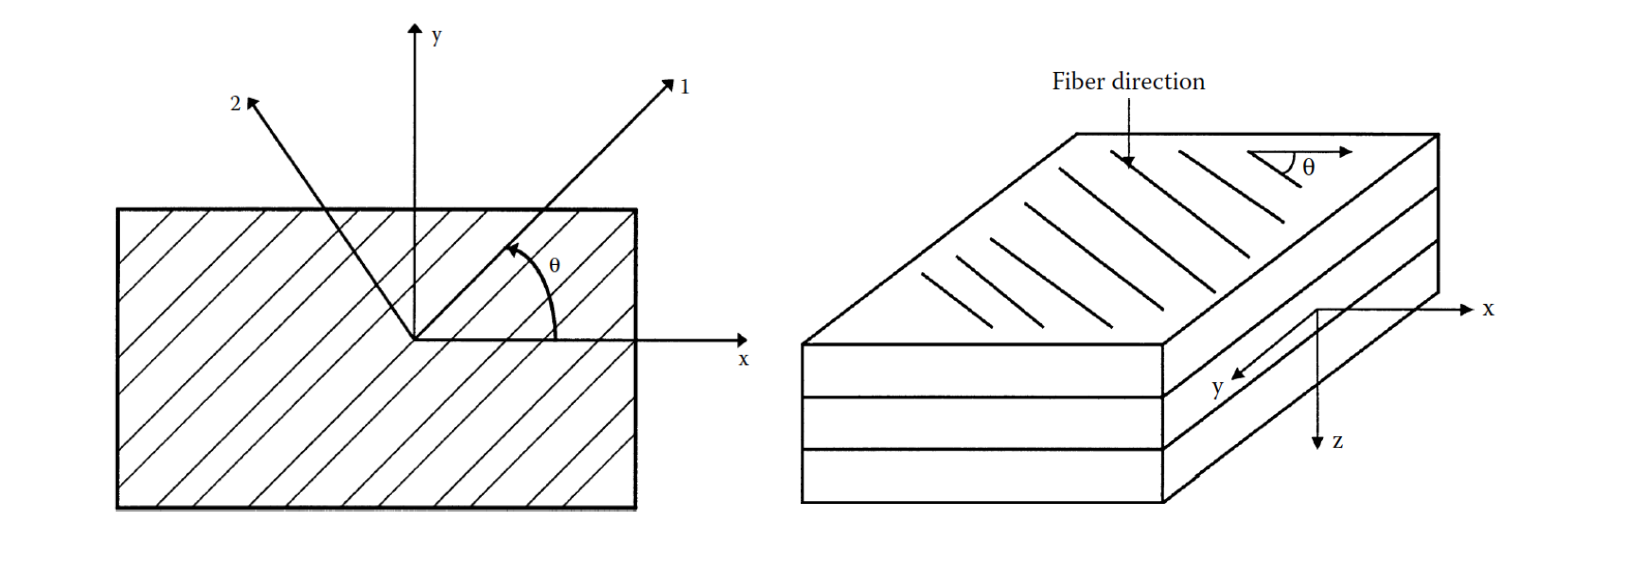
\includegraphics[width=1\linewidth]{fig/lamina_local_global_axes.png}
	\caption{The left diagram shows the local and global axis of an angle lamina, which is from a laminate as shown in the right diagram.}
	\label{fig:lamina_local_and_global}
\end{figure}

A few cases of laminates, such as symmetric laminates, cross-ply laminates, play
an important role in the application of laminated composite material. A laminate
is called an angle ply laminate if it has plies of the same material and
thickness and is only oriented at $+\theta$ and $-\theta$ directions. A model of
an angle ply laminate is as shown in Fig. \ref{fig:angle-ply}.

\begin{figure}[b]
\centering
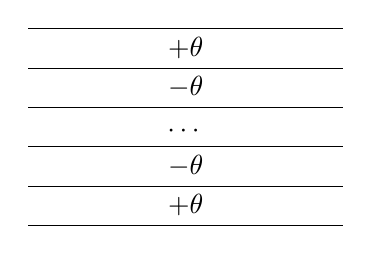
\begin{tikzpicture}
	\draw (0,0) -- (4,0);
	\draw (0,-0.5) -- (4,-0.5) node[midway, above] {$\mathit{+}\theta$};
	\draw (0,-1) -- (4,-1) node[midway, above] {$\mathit{-}\theta$} ;
	\draw (0,-1.5) -- (4,-1.5) node[midway, above] {$\cdots$};
	\draw (0,-2) -- (4,-2) node[midway, above] {$\mathit{-}\theta$};
	\draw (0,-2.5) -- (4,-2.5) node[midway, above] {$\mathit{+}\theta$};
\end{tikzpicture}
\caption{Model for angle ply laminate}
\label{fig:angle-ply}
\end{figure}


\subsubsection{Stress and Strain in a Lamina}
For a single lamina under in-plane loading whose thickness is relatively small,
suppose the upper and lower surfaces of the lamina are free from external
loading. According to Hooke's law, the three-dimensional stress-strain
equations can be reduced to two-dimensional stress-strain equations in the
composite material. The stress-strain relation in local axis 1-2 is
\begin{equation}
	\left[
		\begin{array}{l}
        	\sigma _1\\
        	\sigma _2\\
        	\tau_{12}
    	\end{array}
	\right]
    =
	\left[
		\begin{array}{ccc}
        	Q_{11} & Q_{12} & 0\\
        	Q_{12} & Q_{22} & 0\\
        	0      & 0     & Q_{66}
    	\end{array}
	\right]
	\left[
		\begin{array}{l}
        	\varepsilon_1\\
        	\varepsilon_2\\
			\gamma_{12}
		\end{array} 
	\right]\textstyle{,}
\end{equation}
where $Q_{ij} $ is the stiffness of a lamina. And they are related to
engineering elastic constants as follows:
\begin{equation}
	\begin{array}{l}
		Q_{11}=\frac{E_1}{1-v_{12}v_{21}} \textstyle{,} \\
    	Q_{22}=\frac{E_2}{1-v_{12}v_{21}} \textstyle{,}\\
    	Q_{66}=G_{12} \textstyle{,}\\
    	Q_{12}=\frac{v_{21}E_2}{1-v_{12}v_{21}} \textstyle{,}
    \end{array}
\end{equation}
where $E_1, E_2, v_{12}, G_{12} $ are four independent engineering elastic
constants, which are defined as follows: $E_1 $ is the longitudinal Young's
modulus, $E_2 $ is the transverse Young's modulus, $v_{12} $ is the major
Poisson's ratio, and $G_{12} $ is the in-plane shear modulus.

Stress-strain relation in the global x-y axis is
\begin{equation}
	\label{equ:stress-strain}
	\left[\begin{array}{l}
			\sigma _{x} \\ 
			\sigma _{y} \\
			\tau_{xy}
			\end{array}
	\right]=
	\left[\begin{array}{lll}
			\bar{Q}_{11} & \bar{Q}_{12} & \bar{Q}_{16}\\ 
			\bar{Q}_{12} & \bar{Q}_{22} & \bar{Q}_{26} \\
			\bar{Q}_{16} & \bar{Q}_{26} &\bar{Q}_{66}
		\end{array}
	 \right]
	 \left[\begin{array}{l}
			 \varepsilon_{x} \\ 
	 		 \varepsilon_{y} \\ 
	 		 \gamma_{x y}
	 		\end{array}
	\right] \textstyle{,}
\end{equation}
where
\begin{equation}
	\begin{array}{l}
		\resizebox{.35\textwidth}{!}{$\bar{Q}_{11}=Q_{11} cos^{4}\theta+Q_{22} sin^{4}\theta+2\left(Q_{12}+2
		Q_{66}\right) sin^{2}\theta cos^{2}\theta$}\textstyle{,} \\
		\resizebox{.35\textwidth}{!}{$\bar{Q}_{12}=\left(Q_{11}+Q_{22}-4 Q_{66}\right) sin^{2}\theta
			cos^{2}\theta+Q_{12}\left(cos^{4}\theta+sin^{2}\theta \right)$} \textstyle{,}\\
		\resizebox{.35\textwidth}{!}{$\bar{Q}_{22}=Q_{11} sin^{4}\theta+Q_{22} cos^{4}\theta+2\left(Q_{12}+2
				Q_{66}\right) sin^{2}\theta cos^{2}\theta$}\textstyle{,} \\
		\resizebox{.40\textwidth}{!}{$\bar{Q}_{16}=\left(Q_{11}-Q_{12}-2
			Q_{66}\right) cos^{3}\theta
			sin\theta-\left(Q_{22}-Q_{12}-2Q_{66}\right) sin^{3}\theta cos\theta$} \textstyle{,}\\ 
		\resizebox{.40\textwidth}{!}{$\bar{Q}_{26}=\left(Q_{11}-Q_{12}-2
			Q_{66}\right) cos\theta sin^{3}\theta-\left(Q_{22}-Q_{12}-2
			Q_{66}\right)cos^{3}\theta sin\theta$} \textstyle{,}\\ 
		\resizebox{.40\textwidth}{!}	{$\bar{Q}_{66}=\left(Q_{11}+Q_{22}-2 Q_{12}-2 Q_{66}\right)
			sin\theta^{2}cos\theta^{2}+Q_{66}\left(sin\theta^{4}+cos\theta^{4}\right)$}\textstyle{.}\\
	\end{array}
\end{equation}

\subsubsection{Stress and Strain in a Laminate}
For forces acting on laminates, such as in plate and shell
structures, the relationship between applied forces and displacement
can be given by

\begin{equation} \label{eq:force_and_moments}
	\begin{array}{ll}
	\begin{bmatrix}
		N_x \\
		N_y \\
		N_{xy}
	\end{bmatrix}
	&=
	\begin{bmatrix}
		A_{11} & A_{12} & A_{16} \\
		A_{12} & A_{22} & A_{26} \\
		A_{16} & A_{26} & A_{66} 
	\end{bmatrix}
    \begin{bmatrix}
		\varepsilon_x^0 \\
        \varepsilon_y^0 \\
		\gamma_{xy}^0
    \end{bmatrix}   \\
	&+               
	\begin{bmatrix}
		B_{11} & B_{12} & B_{16} \\
		B_{11} & B_{12} & B_{16} \\
		B_{16} & B_{26} & B_{66} 
	\end{bmatrix}
	\begin{bmatrix}
		k_x \\
		k_y \\
		k_{xy} 
	\end{bmatrix}  \textstyle{,}
	\end{array}
\end{equation}
where $N_x,N_y $ refers to the normal force per unit length;
$N_{xy}$ means shear force per unit length;
$\varepsilon^{0}$ and $k_{xy}$ denotes  mid plane strains and curvature of a laminate in x-y coordinates
The mid-plane strain and curvature is given by
\begin{equation}
    \begin{split}
	&A_{ij}=\sum_{k=1}^{n}(\overline{Q_{ij}})_k(h_k-h_{k-1})  i=1,2,6, j=1,2,6 \textstyle{,}\\
    &B_{ij}=\frac{1}{2}\sum_{k=1}^{n}(\overline{Q_{ij}})_k(h_k^2 - h_{k-1}^2)  i=1,2,6, j=1,2,6\textstyle{,}\\
    &D_{ij}=\frac{1}{3}\sum_{k=1}^{n}(\overline{Q_{ij}})_k(h_k^3 - h_{k-1}^3) i=1,2,6, j=1,2,6\textstyle{.}\\
    \end{split}
\end{equation}

The [A], [B], and [D] matrices are called the extensional, coupling, and bending stiffness matrices,
respectively. The extensional stiffness matrix $[A]$ relates the resultant in-plane forces to the
in-plain strains, and the bending stiffness matrix $[D]$ couples the resultant bending moments to
the plane curvatures.  The coupling stiffness matrix $[B]$ relates the force and moment terms to the
midplane strains and curvatures.

\subsection{Failure criteria for a lamina}

Failure criteria for composite materials are more difficult to predict due to
structural and material complexity. The failure process of composite materials
can be regarded from microscopic and macroscopic points of view. The most
popular criteria about the failure of an angle lamina are from the macroscopic
point of view, which are according to the tensile, compressive, and shear
strengths. As shown in Fig. \ref{fig:failure_surface}, there are two types of failure
criteria\cite{massard1984computer,reddy1987first,fang1993design,soeiro1994multilevel,pelletier2006multi,jadhav2007parametric,omkar2008artificial,choudhury2019failure}
according to failure surfaces. The first failure surface is a rectangle that
includes the maximum stress failure criterion\cite{watkins1987multicriteria},
and maximum strain failure criterion. The second failure surface is ellipsoidal
that includes Tsai-Wu\cite{martin1987optimum,soares1995discrete}, Chamis,
Hoffman, and Hill criteria. In the present study, the two most reliable failure
criteria are adopted, Maximum stress and Tsai-wu. Both these failure criteria
are based on the stress in the local axis instead of principal normal stress and
maximum shear stresses, in which four normal strength parameters and one shear
stress are involved. The five strength parameters are

$(\sigma _1^{T})_{ult}= $ ultimate longitudinal tensile strength(in direction 1),

$(\sigma _1^{C})_{ult}= $ ultimate longitudinal compressive strength,

$(\sigma _2^{T})_{ult}= $ ultimate transverse tensile strength,

$(\sigma _2^{C})_{ult}= $ ultimate transverse compressive strength, and

$(\tau_{12})_{ult}= $ and ultimate in-plane shear strength.

\begin{figure}[b]
\centering
\begin{tikzpicture}
	\begin{scope}
		%\draw[style=help lines] (-3,-3) grid (3,3);
		\draw (0,0) rectangle (2,3);
		\draw[->] (1.3,1.2) -- (2.6,1.2);
		\draw[->] (1.3,1.2) -- (1.3,3.4);
		\node at (2.2,1) {$X_T$};
		\node at (1.5, 3.2) {$Y_T$};
		\node at (-0.2, 0.9) {$X_C$};
		\node at (1.8, -0.2) {$Y_C$};
	\end{scope}
	\begin{scope}[xshift=6cm,yshift=1.15cm]
		%\draw[style=help lines] (-3,-3) grid (3,3);
		\draw[rotate=30] (0,0) ellipse (2cm and 1cm);
		\draw[->] (0.2,0) -- (0.2,2.2);
		\draw[->] (0.2,0) -- (1.9,0);
		\node at (1.6,-0.2) {$X_T$};
		\node at (0.3, 1.3) {$Y_T$};
		\node at (-1.6, 0) {$X_C$};
		\node at (-0.5, -1.5) {$Y_C$};
	\end{scope}
\end{tikzpicture}
\caption{Schematic failure surfaces for maximum stress and quadratic failure
criteria}
\label{fig:failure_surface}
\end{figure}

\subsubsection{Maximum stress(MS) failure criterion}

Maximum stress failure criteria are consist of the normal stress theory and the
shear stress theory. The stress applied to a lamina can be resolved into the
normal stress and shear stress in the local axis. The lamina fails if either of
the normal stress or shear stress in the local axis of a lamina is equal or
exceeds the corresponding ultimate strengths of the unidirectional lamina.  That
is,

\begin{equation}
	\begin{array}{lll}
		\sigma_1 \geq (\sigma _1^{T})_{ult} & \textstyle{ or } &  \sigma_1 \leq -(\sigma _1^{C})_{ult} \textstyle{,} \\
		\sigma_2 \geq (\sigma _2^{T})_{ult} & \textstyle{ or } &   \sigma_2 \leq -(\sigma _2^{C})_{ult} \textstyle{,} \\
		\tau_{12} \geq (\tau_{12})_{ult}    & \textstyle{ or } &     \tau_{12} \leq -(\tau_{12})_{ult}  \textstyle{,}
\end{array}
\end{equation}

where $\sigma_1$ and $\sigma_2$ are the normal stresses in the local axis 1 and 2;
$\tau_{12}$ is the shear stress in the symmetry plane 1-2.

\subsubsection{Tsai-Wu failure criterion}
The Tsai-Wu criterion is one of the most reliable static failure criteria derived from the von
Mises yield criterion.  
A lamina is considered to fail
if \begin{equation} \label{eq:tsai_wu}
\begin{split}
	H_1 \sigma_1  & + H_2 \sigma_2 + H_6 \tau_{12} + H_{11}\sigma_1^2 + H_{22} \sigma_2^2 \\
				  & + H_{66}  \tau_{12}^2 + 2H_{12}\sigma_1\sigma_2 < 1
\end{split}
\end{equation}

is violated, where

\begin{equation}
	\begin{split}
		H_{1}&=\frac{1}{\left(\sigma_{1}^{T}\right)_{u l t}}-\frac{1}{\left(\sigma_{1}^{C}\right)_{u l t}}\textstyle{,} \\
		H_{11}&=\frac{1}{\left(\sigma_{1}^{T}\right)_{u l t}\left(\sigma_{1}^{C}\right)_{u l t}} \textstyle{,}\\
		H_{2}&=\frac{1}{\left(\sigma_{2}^{T}\right)_{u l t}}-\frac{1}{\left(\sigma_{2}^{C}\right)_{u l t}} \textstyle{,}\\
		H_{22}&=\frac{1}{\left(\sigma_{2}^{T}\right)_{u l t}\left(\sigma_{2}^{C}\right)_{u l t}} \textstyle{,}\\
		H_{66}&=\frac{1}{\left(\tau_{12}\right)_{u l t}^{2}} \textstyle{,}\\
		H_{12}&=-\frac{1}{2} \sqrt{\frac{1}{\left(\sigma_{1}^{T}\right)_{u l
		t}\left(\sigma_{1}^{C}\right)_{u l t}\left(\sigma_{2}^{T}\right)_{u l
		t}\left(\sigma_{2}^{C}\right)_{u l t}}}\textstyle{.}
	\end{split}
\end{equation}

$H_i$ is the strength tensor of the second-order; $H_{ij}$ is the strength
tensor of the fourth-order. $\sigma_1$ is the applied normal stress in 
direction 1; $\sigma_2$ is the applied normal stress in direction 2; 
$\tau_{12}$ is the applied in-plane shear stress.




\subsubsection{Strength ratio}
The safety factor, or yield stress, is how much extra load beyond is intended a
composite laminate will take. The strength ratio(SR) is defined as 

\begin{equation}
	\label{eq:sr}S R=\frac{\text {Maximum Load Which Can Be Applied}}{\text {Load Applied}}\textstyle{.}
\end{equation}

\section{Evolutionary Artificial Neural Network}
\begin{figure}[tb]
\centering
	%\resizebox{.7\linewidth}{!}{dd
%\begin{tikzpicture}[show background grid, show background rectangle]
\begin{tikzpicture}
	\useasboundingbox (-3.5,-5.) rectangle (3.5,6.3);
	\scope[transform canvas={scale=1}]
    %\draw[help lines] (-3cm,-7cm) grid (6cm, 5cm);
    \tikzstyle{block} = [rectangle, text centered, draw=black,
    minimum width=1.1cm, minimum height=0.4cm]
	% first level evolution: connection weights
    \node (evaluation-parent) [block, minimum width=2.4cm, minimum
        height=1.8cm,draw=white] {};
    \node (evaluation) [block] at ($(evaluation-parent.north)$) {evaluation};
    \node (reproduction) [block] at ($(evaluation-parent.south)$) {reproduction};
    \node (tasks) [block, minimum width=1.1cm, minimum height=0.4cm] {tasks};

    \draw[->] ($(evaluation.south)+(0.3cm,0cm)$) --
        ($(tasks.north)+(0.3cm,0cm)$) node[auto=left, pos=0.5] {\small weights}; 
    \draw[<-] ($(evaluation.south)+(-0.3cm,0cm)$) --
        ($(tasks.north)+(-0.3cm,0cm)$) node[auto=right, pos=0.5] {\small fitness}; 

	\draw[black] (reproduction.west) -- ++(-0.3cm,0)  |- (evaluation.west);
	\draw[black] (reproduction.east) -- ++(0.3cm,0)   |- (evaluation.east);

    \node (level1) [block,draw=black, minimum width=3.5cm, minimum height=3.0cm] at
        (0cm,0.2cm) {};
    \node [align=left] at ($(level1.north)+(0,-0.2cm)$) {\tiny THE EVOLUTION
        OF};
    \node [align=left] at ($(level1.north)+(0,-0.45cm)$) {\tiny CONNECTION
            WEIGHTS
        };
    % second level evolution: active functions
    \node (level2_container) [block, draw=black, minimum width=5.8cm, minimum
        height=6.0cm] at
        (0, 0.4cm)  {};
    \node [align=left] at ($(level2_container.north)+(0,-0.25cm)$) {\tiny THE EVOLUTION
        OF ACTIVE FUNCTIONS};
    \node (level2-assister) [block, draw=white, minimum width=5cm, minimum
		height=4.6cm] at
        (0, 0.3cm)  {};
    \node (evaluation) [block] at ($(level2-assister.north)$) {\small evaluation of
        active functions};
    \node (reproduction) [block] at ($(level2-assister.south)$) {\small reproduction of
        active functions};

    \draw[->] ($(evaluation.south)+(0.3cm,0cm)$) --
        ($(level1.north)+(0.3cm,0cm)$) node[auto=left, pos=0.5] {\small active functions
        }; 

    \draw[<-] ($(evaluation.south)+(-0.3cm,0cm)$) --
        ($(level1.north)+(-0.3cm,0cm)$) node[auto=right, pos=0.5] {\small fitness}; 

	\draw[black] (reproduction.west) -- ++(-0.3cm,0)  |- (evaluation.west);
	\draw[black] (reproduction.east) -- ++(0.3cm,0)   |- (evaluation.east);
    % third level: evolution of learning rules
    \node (level3-assister) [block, draw=white, minimum width=3cm, minimum
        height=7.6cm] at
        (0, 0.4cm)  {};
	\node (level3_container) [block, draw=black, minimum width=7.5cm, minimum
		height=9cm] at (0, 0.4cm)  {};
    \node [align=left] at ($(level3_container.north)+(0,-0.25cm)$) {\tiny THE EVOLUTION
        OF LEARNING RULES};
    \node (evaluation) [block] at   ($(level3-assister.north)$) {\small evaluation of
        learning rules};
    \node (reproduction) [block] at ($(level3-assister.south)$) {\small reproduction of
        learning rules};
    \draw[->] ($(evaluation.south)+(0.3cm,0cm)$) --
        ($(level2_container.north)+(0.3cm,0cm)$) node[auto=left, pos=0.5] {\small learning
        rule}; 
    \draw[<-] ($(evaluation.south)+(-0.3cm,0cm)$) --
        ($(level2_container.north)+(-0.3cm,0cm)$) node[auto=right, pos=0.5] {\small fitness}; 

	\draw[black] (reproduction.west) -- ++(-0.9cm,0)  |- (evaluation.west);
	\draw[black] (reproduction.east) -- ++(0.9cm,0)   |- (evaluation.east);

	% fourth level: evolution of topology
    \node (level4-assister) [block, draw=white, minimum width=3cm, minimum
        height=11cm] at
        (0, 0.8cm)  {};
	\node (level4_container) [block, draw=black, minimum width=9cm, minimum
		height=11.8cm] at (0, 0.8cm)  {};
    \node (evaluation) [block] at   ($(level4-assister.north)$) {\small evaluation of
        topology};
    \node (reproduction) [block] at ($(level4-assister.south)$) {\small reproduction of
        topology};
    \draw[->] ($(evaluation.south)+(0.3cm,0cm)$) --
        ($(level3_container.north)+(0.3cm,0cm)$) node[auto=left, pos=0.5] {\small learning
        topology}; 
    \draw[<-] ($(evaluation.south)+(-0.3cm,0cm)$) --
        ($(level3_container.north)+(-0.3cm,0cm)$) node[auto=right, pos=0.5] {\small fitness}; 
	\draw[black] (reproduction.west) -- ++(-2.1cm,0)  |- (evaluation.west);
	\draw[black] (reproduction.east) -- ++(2.1cm,0)   |- (evaluation.east);

    %\node (evaluation) [block] at ($(level3-assister.north)$) {\small evaluation of
    %    architecture};
    %\node (reproduction) [block] at ($(level3-assister.south)$) {\small reproduction of
    %    learning architecture};
    % level 6
    %\node (level6) [block, minimum width=7.0cm, minimum
    %    height=8.1cm] at
    %    (0, 0.5cm)  {};
    %\node [align=left] at ($(level6.north)+(0,-0.2cm)$) {\tiny THE EVOLUTION OF
    %        ARCHITECTURE
    %    };
	\endscope
\end{tikzpicture}
%}
\caption{A general framwwork for EANN, in which fitness refers to the corresponding value of objective function.}
\label{fig:evolution}
\end{figure}


\subsection{General neural network}
In this paper, the feedforward ANN is adopted in the current
study, since it is straightforward and simple to code. For function
approximation through an ANN, Cybenko demonstrated that a two-layer perceptron
can form an arbitrarily close approximation to any continuous nonlinear
mapping\cite{cybenko1989approximation}. Therefore, a two-layer feedforward ANN
is proposed in the present study. Fig. \ref{fig:gnn} shows a general framework for a
two-layer NN, in which the number of nodes in the hidden layer and the
connection with inputs, are critical in the design of an ANN. For nodes in the
hidden layer, we can think of them as feature extractors or detectors.
Therefore, nodes within it should partially be connected with the inputs of an ANN,
since the unnecessary connections would increase the model's complicacy, which
will reduce an ANN’s performance. Because we treat the nodes in the hidden layer
as feature extractors, so the number of nodes in this layer should be less than
the number of inputs. For the nodes in the last layer, every node should be
fully connected with nodes in the previous layer, since we think of the nodes
in the hidden layer as features. The rest, which affects a NN’s performance,
are activation function, and ANN's training method. In the following section, we
denote the $i$th node in the input layer, and the hidden layer, as $i_i$, and $h_i$,
respectively.

\begin{figure}
	\centering
	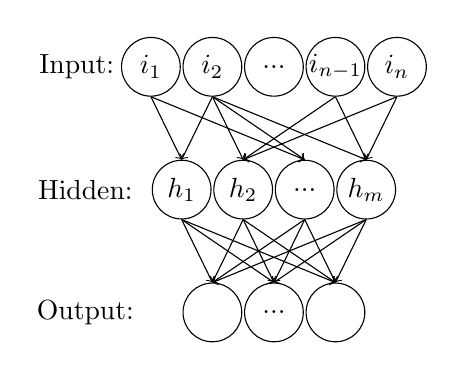
\begin{tikzpicture}
		[ plain/.style={ draw=none, fill=none, }, remember picture, net/.style={ matrix of nodes, nodes={ draw, circle,
			inner sep=7.5pt
			},
		  nodes in empty cells,
		  column sep=-10.5pt,
		  row sep=0.8cm
		  }
		]
	%\draw[help lines] (-3cm,-6cm) grid (6cm,3cm);
	\matrix[net] (mat)
		{
				  & |[plain]| &           & |[plain]|  &           & |[plain]| &           &  |[plain]|      &               \\
		|[plain]| &           & |[plain]| &            & |[plain]| &           & |[plain]| &                 & |[plain]|     \\ 
		|[plain]| & |[plain]| &           & |[plain]|  &           & |[plain]| & 	  	   &  |[plain]|      & |[plain]|     \\ 
	  };

	  \node at ($(mat-1-1.west)+(-16pt,0)$) {Input: };
	  \node at ($(mat-2-2.west)+(-24pt,0)$) {Hidden:};
	  \node at ($(mat-3-2.west)+(-24pt,0)$) {Output:};
	  \node at (mat-1-1.base) {$i_1$};
	  \node at (mat-1-3.base) {$i_2$};
	  \node at (mat-1-5.base) {...};
	  \node at (mat-1-7.base) {$i_{n-1}$};
	  \node at (mat-1-9.base) {$i_{n}$};
	  \node at (mat-2-2.base) {$h_1$};
	  \node at (mat-2-4.base) {$h_2$};
	  \node at (mat-2-6.base) {$...$};
	  \node at (mat-2-8.base) {$h_{m}$};
	  \node at (mat-3-5.base) {$...$};

		 \foreach \a in {1,3}{
			\foreach \b in {2,6}{
				\draw[->] (mat-1-\a.south) -- (mat-2-\b.north);
			 }
		  }
		 \foreach \a in {3,7,9}{
			\foreach \b in {4,8}{
				\draw[->] (mat-1-\a.south) -- (mat-2-\b.north);
			 }
		  }

		 \foreach \c in {2,4,6,8}{
			\foreach \d in {3,5,7}{
				\draw[->] (mat-2-\c.south) -- (mat-3-\d.north);
			}
	 }
\end{tikzpicture}
\caption{General Neural Network}
\label{fig:gnn}
\end{figure}





\subsection{Activation function}

The activation function is one of the critical parts of an ANN. Liu
\cite{liu1996evolutionary} et al. claims that the performance of neural networks with
different activation functions is different, even if they have the same
architecture.  A generalized activation function can be written as

\begin{equation}
	y_i = f_i(\sum_{j=1}^n{w_{ij}x_j - \theta})
\end{equation}

where $y_i$ is the output of the node $i$, $x_j$ is the $j$th input to the
node, and $w_{ij}$ is the connection weight between adjacent nodes $i$ and $j$.
Tab. \ref{tab:transfer_function} displays the most widely adopted activation
functions in the design of an ANN, which is used for the current study.

\begin{table*}[!t]
\centering
\caption{Different Activation Functions}
\label{tab:active_function}
\begin{adjustbox}{width=1\textwidth}
\label{tab:transfer_function}
	\begin{tabular}{lllc}
			\toprule
			Type & Description  & Formula & Range  \\
			\midrule
			Linear   & The output is proportional to the input & $f(x)=cx$                  &  $(-\infty, +\infty)$ \\
			Sigmoid  & A family of S-shaped functions          & $f(x)=\frac{1}{1+e^{-cx}}$ & $(0, 1)$ \\
			tanh     & A family of Hyperbloic functions        & $f(x)=\frac{e^x -e^{-x}}{e^x+e^{-x}}$ & $(0, 1)$ \\
			Gaussian & A coninuous bell-shaped curve           & $f(x)=e^{-x^2}$            & $(0,1)$ \\ 
			ReLU     & A piece-wise function                   & $f(x)= max{0,x}$           & $(0, +\infty)$ \\
			Softplus & A family of S-shaped functions          & $f(x) = ln(1+e^x)$         & $(0, +\infty)$ \\
			\bottomrule
	\end{tabular}
\end{adjustbox}
\end{table*}


\subsection{Weights learning}
The weight training in an ANN is to minimize the error function, such as the
most widely used mean square error function, which calculates the difference
between the desired and the prediction output values averaged overall examples.
Gradient descent algorithm is widely adopted to reduce the value of an error
function, which has been successfully applied in many practical areas. However,
this class of algorithms is plagued by the possible existence of local minima
or ”flat spots” and ”the curse of dimensionality.” One method to overcome this
problem is to adopt a genetic algorithm(GA)


\begin{figure*}
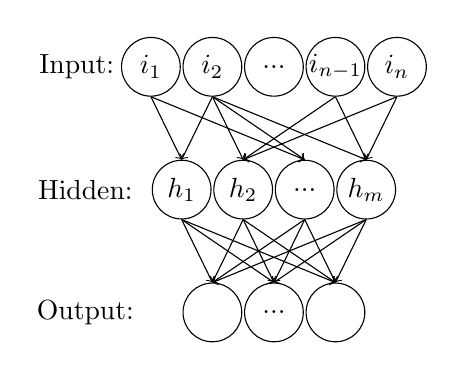
\begin{tikzpicture}
[ plain/.style={ draw=none, fill=none, }, remember picture, net/.style={ matrix of nodes, nodes={ draw, circle,
    inner sep=7.5pt
    },
  nodes in empty cells,
  column sep=-10.5pt,
  row sep=0.8cm
  }
]
%\draw[help lines] (-3cm,-6cm) grid (6cm,3cm);
\matrix[net] (mat)
{
              & |[plain]| &           & |[plain]|  &           & |[plain]| &           &  |[plain]|      &               \\
    |[plain]| &           & |[plain]| &            & |[plain]| &           & |[plain]| &                 & |[plain]|     \\ 
    |[plain]| & |[plain]| &           & |[plain]|  &           & |[plain]| & 	  	   &  |[plain]|      & |[plain]|     \\ 
  };

  \node at ($(mat-1-1.west)+(-16pt,0)$) {Input: };
  \node at ($(mat-2-2.west)+(-24pt,0)$) {Hidden:};
  \node at ($(mat-3-2.west)+(-24pt,0)$) {Output:};
  \node at (mat-1-1.base) {$i_1$};
  \node at (mat-1-3.base) {$i_2$};
  \node at (mat-1-5.base) {...};
  \node at (mat-1-7.base) {$i_{n-1}$};
  \node at (mat-1-9.base) {$i_{n}$};
  \node at (mat-2-2.base) {$h_1$};
  \node at (mat-2-4.base) {$h_2$};
  \node at (mat-2-6.base) {$...$};
  \node at (mat-2-8.base) {$h_{m}$};
  \node at (mat-3-5.base) {$...$};

 \foreach \a in {1,3}{
    \foreach \b in {2,6}{
        \draw[->] (mat-1-\a.south) -- (mat-2-\b.north);
     }
  }
 \foreach \a in {3,7,9}{
    \foreach \b in {4,8}{
        \draw[->] (mat-1-\a.south) -- (mat-2-\b.north);
     }
  }

 \foreach \c in {2,4,6,8}{
    \foreach \d in {3,5,7}{
 		\draw[->] (mat-2-\c.south) -- (mat-3-\d.north);
	}
 }
\end{tikzpicture}
\caption{Neural Network Model}
\end{figure*}



\begin{figure}
\centering
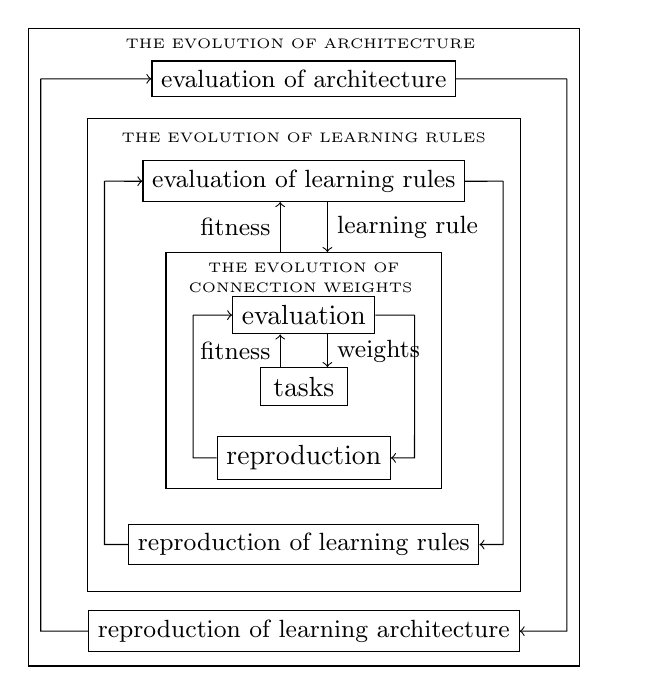
\begin{tikzpicture}
    %\draw[help lines] (-3cm,-6cm) grid (6cm, 6cm);
    \tikzstyle{block} = [rectangle, text centered, draw=black,
    minimum width=1.1cm, minimum height=0.4cm]
    % first level
    \node (evaluation-parent) [block, minimum width=2.4cm, minimum
        height=1.8cm,draw=white] {};
    \node (evaluation) [block] at ($(evaluation-parent.north)$) {evaluation};
    \node (reproduction) [block] at ($(evaluation-parent.south)$) {reproduction};
    \node (tasks) [block, minimum width=1.1cm, minimum height=0.4cm] {tasks};

    \draw[->] ($(evaluation.south)+(0.3cm,0cm)$) --
        ($(tasks.north)+(0.3cm,0cm)$) node[auto=left, pos=0.5] {\small weights}; 
    \draw[<-] ($(evaluation.south)+(-0.3cm,0cm)$) --
        ($(tasks.north)+(-0.3cm,0cm)$) node[auto=right, pos=0.5] {\small fitness}; 

    % get intersection
    \draw[white] (evaluation.west) coordinate (A) -- ++(-1.5cm,0) coordinate (B);
    \draw[white] (reproduction.west) -- ++(-0.3cm,0) coordinate (C) -- ++(0,4cm) coordinate
        (D);
    \draw[black] (reproduction.west) -- ++(-0.3cm,0) -- (intersection cs:
        first line={(A)--(B)}, second line={(C)--(D)}) coordinate (E);
    \draw[->] (E) -- (evaluation.west);

    \draw[white] (evaluation.east) coordinate (E) -- ++(2cm,0) coordinate (F);
    \draw[white] (reproduction.east) -- ++(0.3cm,0) coordinate (G) -- ++(0,4cm) coordinate
        (H);
    \draw[<-] (reproduction.east) -- ++(0.3cm,0) -- (intersection cs:
        first line={(E)--(F)}, second line={(G)--(H)}) coordinate (I);
    \draw (I) -- (evaluation.east);

    % second level
    \node (level2) [block,draw=black, minimum width=3.5cm, minimum height=3.0cm] at
        (0cm,0.2cm) {};
    \node [align=left] at ($(level2.north)+(0,-0.2cm)$) {\tiny THE EVOLUTION
        OF};
    \node [align=left] at ($(level2.north)+(0,-0.45cm)$) {\tiny CONNECTION
            WEIGHTS 
        };
    % third level
    \node (level3-assister) [block, draw=white, minimum width=5cm, minimum
		height=4.6cm] at
        (0, 0.3cm)  {};
    \node (evaluation) [block] at ($(level3-assister.north)$) {\small evaluation of
        learning rules};
    \node (reproduction) [block] at ($(level3-assister.south)$) {\small reproduction of
        learning rules};

    \draw[->] ($(evaluation.south)+(0.3cm,0cm)$) --
        ($(level2.north)+(0.3cm,0cm)$) node[auto=left, pos=0.5] {\small learning
        rule}; 
    \draw[<-] ($(evaluation.south)+(-0.3cm,0cm)$) --
        ($(level2.north)+(-0.3cm,0cm)$) node[auto=right, pos=0.5] {\small fitness}; 

    \draw[white] (evaluation.west) coordinate (A) -- ++(-1.3cm,0) coordinate (B);
    \draw[white] (reproduction.west) -- ++(-0.3cm,0) coordinate (C) -- ++(0,4cm) coordinate
        (D);
    \draw[black] (reproduction.west) -- ++(-0.3cm,0) -- (intersection cs:
        first line={(A)--(B)}, second line={(C)--(D)}) coordinate (E);
    \draw[->] (E) -- (evaluation.west);

    \draw[white] (evaluation.east) coordinate (E) -- ++(2cm,0) coordinate (F);
    \draw[white] (reproduction.east) -- ++(0.3cm,0) coordinate (G) -- ++(0,4cm) coordinate
        (H);
    \draw[<-] (reproduction.east) -- ++(0.3cm,0) -- (intersection cs:
        first line={(E)--(F)}, second line={(G)--(H)}) coordinate (I);
    \draw (I) -- (evaluation.east);
   % fourth level
    \node (level4) [block, draw=black, minimum width=5.5cm, minimum
        height=6.0cm] at
        (0, 0.4cm)  {};
    \node [align=left] at ($(level4.north)+(0,-0.25cm)$) {\tiny THE EVOLUTION
        OF LEARNING RULES};
    % level five
    \node (level5-assister) [block, draw=white, minimum width=6.4cm, minimum
        height=7.0cm] at
        (0, 0.4cm)  {};
    \node (evaluation) [block] at ($(level5-assister.north)$) {\small evaluation of
        architecture};
    \node (reproduction) [block] at ($(level5-assister.south)$) {\small reproduction of
        learning architecture};

    \draw[white] (evaluation.west) coordinate (A) -- ++(-1.5cm,0) coordinate (B);
    \draw[white] (reproduction.west) -- ++(-0.6cm,0) coordinate (C) -- ++(0,4cm) coordinate
        (D);
    \draw[black] (reproduction.west) -- ++(-0.6cm,0) -- (intersection cs:
        first line={(A)--(B)}, second line={(C)--(D)}) coordinate (E);
    \draw[->] (E) -- (evaluation.west);

    \draw[white] (evaluation.east) coordinate (E) -- ++(2cm,0) coordinate (F);
    \draw[white] (reproduction.east) -- ++(0.6cm,0) coordinate (G) -- ++(0,4cm) coordinate
        (H);
    \draw[<-] (reproduction.east) -- ++(0.6cm,0) -- (intersection cs:
        first line={(E)--(F)}, second line={(G)--(H)}) coordinate (I);
    \draw (I) -- (evaluation.east);
    % level 6
    \node (level6) [block, minimum width=7.0cm, minimum
        height=8.1cm] at
        (0, 0.5cm)  {};
    \node [align=left] at ($(level6.north)+(0,-0.2cm)$) {\tiny THE EVOLUTION OF
            ARCHITECTURE
        };
\end{tikzpicture}
\caption{Genetic algorithm and artificial neural network}
\end{figure}


\section{Experiment}
We applied this search strategy to dataset generated by the classic lamination
theory and failure theories. In this dataset, sixtheen attribues and two actual
values are given.

\subsection{Dataset Preparation}
Equation \ref{equ:stress-strain} takes an analytical approach to model the
relationship between stress and strain. We sample this function to yield 14000 points
uniformly distributed over the domain space.

The range of in-plane loading is from 0 to 120; the range of fiber orientation $\theta$ is from
-90 to 90; ply thickness $t$ is 1.27mm, number of plies range $N$ is from 4 to 120;
Three different material is used in this experiment, as shown in table \ref{tab:mat}.
Figure \ref{tab:traing-data} shows part of the training data.

In order to speeds up the learning and accerlate convergence, the input
atttributes of the data set are rescaled to between 0 and 1.0 by a linear function.

\begin{table}	
\label{tab:traing-data}
		\resizebox{\textwidth}{!}{
	\begin{tabular}{cccc|cc}
		\toprule
		\multicolumn{4}{c}{\textbf{Input}} &  \multicolumn{2}{c}{\textbf{Output}} \\
		\midrule
		Load  &  \makecell{Laminate \\ Structure }  & \makecell{Material \\ Property} & \makecell{Failure \\  Property}  & MS & Tsai-Wu \\
		\midrule

		-70,-10,-40,  & 90,-90,4,1.27, & 38.6,8.27,0.26,4.14,  & 1062.0,610.0,31,118,72,  & 0.0102, & 0.0086 \\
		-10,10,0,     & -86,86,80,1.27,& 181.0,10.3,0.28,7.17, & 1500.0,1500.0,40,246,68, & 0.4026, & 2.5120 \\
		-70,-50,80,   & -38,38,4,1.27, & 116.6,7.67,0.27,4.173,& 2062.0,1701.0,70,240,105,& 0.0080, & 0.0325 \\
		-70,80,-40,   & 90,-90,48,1.27,& 38.6,8.27,0.26,4.14,  & 1062.0,610.0,31,118,72,  & 0.0218, & 0.1028 \\
		-20,-30,0,    & -86,86,60,1.27,& 181.0,10.3,0.28,7.17, & 1500.0,1500.0,40,246,68, & 0.6481, & 0.9512 \\
		0,-40,0,      & 74,-74,168,1.27,& 181.0,10.3,0.28,7.17,& 1500.0,1500.0,40,246,68, & 1.3110, & 3.9619 \\
		\bottomrule
		\end{tabular}
	}
\end{table}

\begin{table*}[ht]
\caption{Comparison of the carbon/epoxy, graphite/epoxy, and glass/epoxy properties}
\centering
\begin{adjustbox}{width=1\textwidth}
\label{tab:mat}
\begin{tabular}{cccccc}
\toprule
Property								   & Symbol				  & Unit  &  Carbon/Epoxy&  Graphite/Epoxy  &  Glass/Epoxy   \\
\midrule
Longitudinal elastic modulus			   & $E_1$				  & GPa   &  116.6       &  181             &  38.6           \\
Traverse elastic modulus				   & $E_2$				  & GPa   &  7.67        &  10.3            &  8.27           \\
Major Poisson's ratio					   & $v_{12}$			  &       &  0.27        &  0.28            &  0.26           \\
Shear modulus							   & $G_{12}$			  & GPa   &  4.17        &  7.17            &  4.14           \\
Ultimate longitudinal tensile strength     & $(\sigma_1^T)_{ult}$ & MP    &  2062        &  1500            &  1062            \\
Ultimate longitudinal compressive strength & $(\sigma_1^C)_{ult}$ & MP    &  1701        &  1500            &  610             \\
Ultimate transverse tensile strength       & $(\sigma_2^T)_{ult}$ & MPa   &  70          &  40              &  31              \\
Ultimate transverse compressive strength   & $(\sigma_2^C)_{ult}$ & MPa   &  240         &  246             &  118              \\
Ultimate in-plane shear strength           & $(\tau_{12})_{ult}$  & MPa   &  105         &  68              &  72               \\
Density                                    & $\rho$               & $g/cm^3$ &  1.605    &  1.590           &  1.903               \\
Cost                                       &                      &       &  8           &  2.5             &  1               \\
\bottomrule
\end{tabular}
\end{adjustbox}
\end{table*}


\begin{figure}[h!]
	\centering
	\begin{subfigure}[b]{1.0\linewidth}
		\centering
		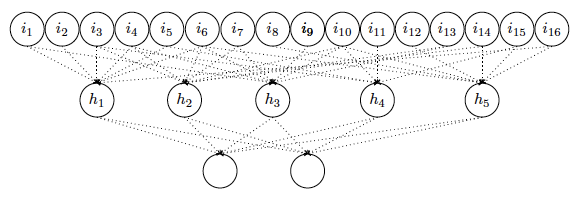
\includegraphics[width=0.8\textwidth]{./a0_figure_ann_for_clt_architecture_example1.png}
		\caption{Parent 1}
		\label{fig:p1}
	\end{subfigure}
	\newline
	\begin{subfigure}[b]{1.0\linewidth}
		\centering
		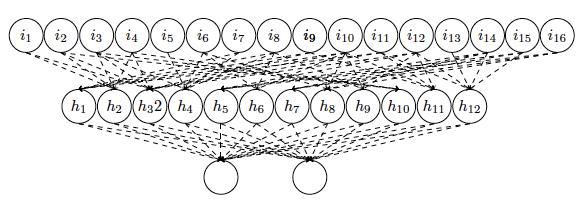
\includegraphics[width=0.8\textwidth]{./a0_figure_ann_for_clt_architecture_example2.png}
		\caption{Parent 2}
		\label{fig:p2}
	\end{subfigure}
	\newline
	\begin{subfigure}[b]{1.0\linewidth}
		\centering
		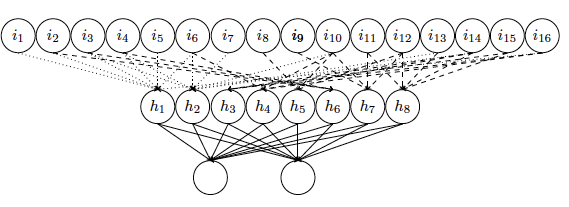
\includegraphics[width=0.8\textwidth]{./a0_figure_ann_for_clt_architecture_child.png}
		\caption{Child}
		\label{fig:child}
	\end{subfigure}
	\caption{Search Operation}
	\label{fig:search}
\end{figure}

\begin{figure*}
\centering
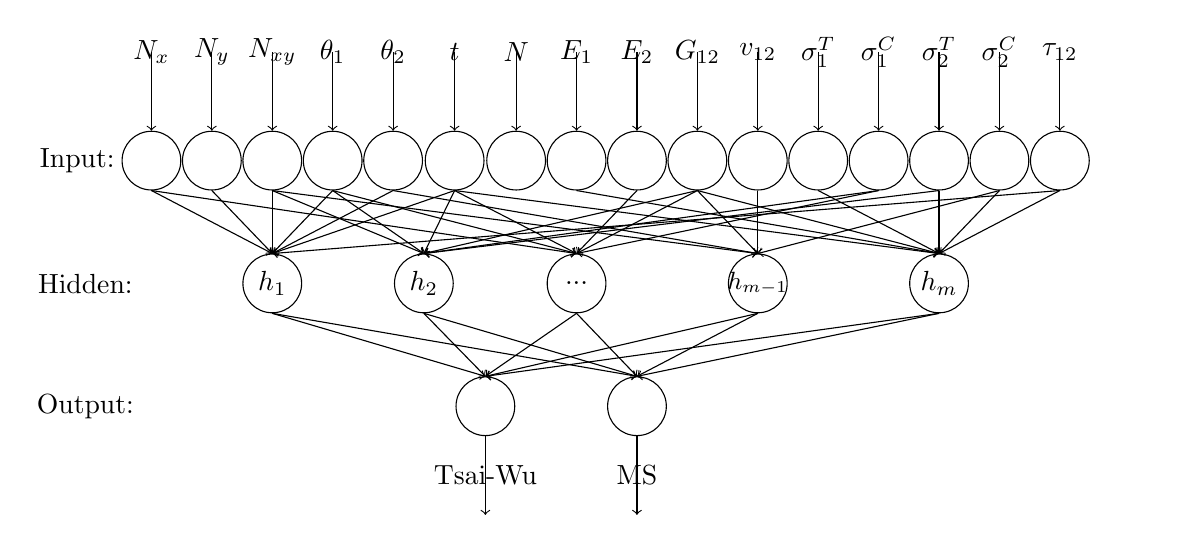
\begin{tikzpicture}
[ p/.style={ draw=none, fill=none, }, remember picture, 
  net/.style={ matrix of nodes, nodes={ draw, circle, inner sep=7.5pt },
  nodes in empty cells,
  column sep=-10.5pt,
  row sep=0.8cm
  }
]
%\draw[help lines] (-3cm,-6cm) grid (6cm,3cm);
\matrix[net] (mat)
{
	  & |[p]| &  & |[p]| &  & |[p]| &  & |[p]| &  & |[p]| &  & |[p]| &  & |[p]| &  & |[p]| &  &
	    |[p]| &  & |[p]| &  & |[p]| &  & |[p]| &  & |[p]| &  & |[p]| &  & |[p]| &  & |[p]|    \\
 |[p]| & |[p]| & |[p]| &  |[p]| &        & |[p]| & |[p]| & |[p]| &|[p]| &       & |[p]| &  |[p]| & |[p]| &
 |[p]| &       & |[p]| &  |[p]| &  |[p]| & |[p]| & |[p]| &       &|[p]| & |[p]| & |[p]| & |[p]|
	   & |[p]| &       &  |[p]| &  |[p]| & |[p]| & |[p]| & |[p]| &|[p]| \\ 
 |[p]| &  |[p]| & |[p]|  &  |[p]| & |[p]|  &  |[p]| &  |[p]| &  |[p]| & |[p]| & |[p]| & |[p]| &       & |[p]|
	   &  |[p]| & |[p]|  &  |[p]| &        &  |[p]| &  |[p]| &  |[p]| & |[p]| & |[p]| & |[p]| & |[p]| &     |[p]|
	   &  |[p]| & |[p]|  &  |[p]| & |[p]|  &  |[p]| &  |[p]| &  |[p]| \\ 
  };
  \draw[<-] (mat-1-1.north) --  ++(0,1) node {$N_x$};
  \draw[<-] (mat-1-3.north) --  ++(0,1) node {$N_y$};
  \draw[<-] (mat-1-5.north) --  ++(0,1) node {$N_{xy}$};
  \draw[<-] (mat-1-7.north) --  ++(0,1) node {$\theta_1$};
  \draw[<-] (mat-1-9.north) --  ++(0,1) node {$\theta_2$};
  \draw[<-] (mat-1-11.north) --  ++(0,1) node {$t$};
  \draw[<-] (mat-1-13.north) --  ++(0,1) node {$N$};
  \draw[<-] (mat-1-15.north) --  ++(0,1) node {$E_1$};
  \draw[<-] (mat-1-17.north) --  ++(0,1) node {$E_2$};
  \draw[<-] (mat-1-19.north) --  ++(0,1) node {$G_{12}$};
  \draw[<-] (mat-1-21.north) --  ++(0,1) node {$v_{12}$};
  \draw[<-] (mat-1-23.north) --  ++(0,1) node {$\sigma_1^T$};
  \draw[<-] (mat-1-25.north) --  ++(0,1) node {$\sigma_1^C$};
  \draw[<-] (mat-1-27.north) --  ++(0,1) node {$\sigma_2^T$};
  \draw[<-] (mat-1-29.north) --  ++(0,1) node {$\sigma_2^C$};
  \draw[<-] (mat-1-31.north) --  ++(0,1) node {$\tau_{12}$};
  \draw[->] (mat-3-12.south) --  ++(0,-1) node[pos=0.5, swap] {Tsai-Wu};
  \draw[->] (mat-3-17.south) --  ++(0,-1) node[pos=0.5, swap] {MS};
  \node at ($(mat-1-1.west)+(-16pt,0)$) {Input: };
  \node at ($(mat-2-2.west)+(-24pt,0)$) {Hidden:};
  \node at ($(mat-3-2.west)+(-24pt,0)$) {Output:};
  \node at (mat-2-5.base) {$h_1$};
  \node at (mat-2-10.base) {$h_2$};
  \node at (mat-2-15.base) {$...$};
  \node at (mat-2-21.base) {\small{$h_{m-1}$}};
  \node at (mat-2-27.base) {$h_{m}$};
 \foreach \a in {1,3,5,7,9,11,31}{
        \draw[->] (mat-1-\a.south) -- (mat-2-5.north);
     }
 \foreach \a in {5,7,11,19,25,27}{
        \draw[->] (mat-1-\a.south) -- (mat-2-10.north);
     }
 \foreach \a in {1,7,11,17,19,25}{
        \draw[->] (mat-1-\a.south) -- (mat-2-15.north);
     }
 \foreach \a in {5,9,19,21,29}{
        \draw[->] (mat-1-\a.south) -- (mat-2-21.north);
     }
 \foreach \a in {11,15,19,23,27,29,31}{
        \draw[->] (mat-1-\a.south) -- (mat-2-27.north);
     }
 \foreach \c in {5,10,15,21,27}{
    \foreach \d in {12,17}{
 		\draw[->] (mat-2-\c.south) -- (mat-3-\d.north);
	}
 }
\end{tikzpicture}
\caption{Neural Network Model}
\end{figure*}



The inputs of the neural network is consist of four parts: in-plane loading
$N_x$, $N_y$, and $N_{xy}$, design parameters of laminate, two distinct fiber
orientation angle $\theta_1$ and $\theta_2$, ply thickness $t$, total number of
plies $N$; five engineering constants of composite materials, $E_1$, $E_2$, ;
five strength parameters of a unidirectional lamina. There are two outputs in
the neural network, safety factors for MS theory and Tsai-Wu theory, respectively.

\begin{figure}
\centering
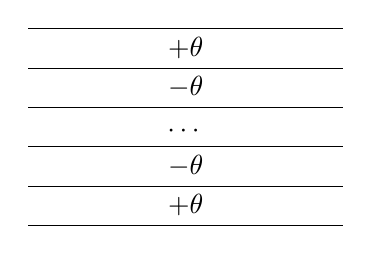
\begin{tikzpicture}
	\draw (0,0) -- (4,0);
	\draw (0,-0.5) -- (4,-0.5) node[midway, above] {$\mathit{+}\theta$};
	\draw (0,-1) -- (4,-1) node[midway, above] {$\mathit{-}\theta$} ;
	\draw (0,-1.5) -- (4,-1.5) node[midway, above] {$\cdots$};
	\draw (0,-2) -- (4,-2) node[midway, above] {$\mathit{-}\theta$};
	\draw (0,-2.5) -- (4,-2.5) node[midway, above] {$\mathit{+}\theta$};
\end{tikzpicture}
\caption{Model for Angle ply laminate}
\end{figure}






\section{Conclusion}
We review the use of genetic algorithms and artificial neural networks as an
alternative approach for calculating the strength ratio of an angle ply
laminate under in-plane loading, traditionally, which is obtained through CLT,
and corresponding failure theories, such as Maximum stress theory and Tsai-wu
failure theory. To obtain optimal architecture, we propose a two-layer ANN
framework and four levels of evolution on the design of ANN.  It was
demonstrated that ANN is an efficient and simple tool to compute the strength
ratio, instead of the complex analytical mathematical model. Our findings
underline the practical applicability of ANN on the analysis of composite
material.  



\section{Acknowledgment}
The work has partly been supported by the work supported by China Scholarship
Council(CSC) under grant no. 201806630112


%\bibliographystyle{plain}
\bibliographystyle{IEEEtran}
\bibliography{src/a5_reference}


% Note that \label must occur AFTER (or within) \caption.
% For figures, \caption should occur after the \includegraphics.
% Note that IEEEtran v1.7 and later has special internal code that
% is designed to preserve the operation of \label within \caption
% even when the captionsoff option is in effect. However, because
% of issues like this, it may be the safest practice to put all your
% \label just after \caption rather than within \caption{}.
%
% Reminder: the "draftcls" or "draftclsnofoot", not "draft", class
% option should be used if it is desired that the figures are to be
% displayed while in draft mode.
%
%\begin{figure}[!t]
%\centering
%\includegraphics[width=2.5in]{myfigure}
% where an .eps filename suffix will be assumed under latex, 
% and a .pdf suffix will be assumed for pdflatex; or what has been declared
% via \DeclareGraphicsExtensions.
%\caption{Simulation Results}
%\label{fig_sim}
%\end{figure}

% Note that IEEE typically puts floats only at the top, even when this
% results in a large percentage of a column being occupied by floats.


% An example of a double column floating figure using two subfigures.
% (The subfig.sty package must be loaded for this to work.)
% The subfigure \label commands are set within each subfloat command, the
% \label for the overall figure must come after \caption.
% \hfil must be used as a separator to get equal spacing.
% The subfigure.sty package works much the same way, except \subfigure is
% used instead of \subfloat.
%
%\begin{figure*}[!t]
%\centerline{\subfloat[Case I]\includegraphics[width=2.5in]{subfigcase1}%
%\label{fig_first_case}}
%\hfil
%\subfloat[Case II]{\includegraphics[width=2.5in]{subfigcase2}%
%\label{fig_second_case}}}
%\caption{Simulation results}
%\label{fig_sim}
%\end{figure*}
%
% Note that often IEEE papers with subfigures do not employ subfigure
% captions (using the optional argument to \subfloat), but instead will
% reference/describe all of them (a), (b), etc., within the main caption.


% An example of a floating table. Note that, for IEEE style tables, the 
% \caption command should come BEFORE the table. Table text will default to
% \footnotesize as IEEE normally uses this smaller font for tables.
% The \label must come after \caption as always.
%
%\begin{table}[!t]
%% increase table row spacing, adjust to taste
%\renewcommand{\arraystretch}{1.3}
% if using array.sty, it might be a good idea to tweak the value of
% \extrarowheight as needed to properly center the text within the cells
%\caption{An Example of a Table}
%\label{table_example}
%\centering
%% Some packages, such as MDW tools, offer better commands for making tables
%% than the plain LaTeX2e tabular which is used here.
%\begin{tabular}{|c||c|}
%\hline
%One & Two\\
%\hline
%Three & Four\\
%\hline
%\end{tabular}
%\end{table}


% Note that IEEE does not put floats in the very first column - or typically
% anywhere on the first page for that matter. Also, in-text middle ("here")
% positioning is not used. Most IEEE journals/conferences use top floats
% exclusively. Note that, LaTeX2e, unlike IEEE journals/conferences, places
% footnotes above bottom floats. This can be corrected via the \fnbelowfloat
% command of the stfloats package.



% trigger a \newpage just before the given reference
% number - used to balance the columns on the last page
% adjust value as needed - may need to be readjusted if
% the document is modified later
%\IEEEtriggeratref{8}
% The "triggered" command can be changed if desired:
%\IEEEtriggercmd{\enlargethispage{-5in}}

% references section

% can use a bibliography generated by BibTeX as a .bbl file
% BibTeX documentation can be easily obtained at:
% http://www.ctan.org/tex-archive/biblio/bibtex/contrib/doc/
% The IEEEtran BibTeX style support page is at:
% http://www.michaelshell.org/tex/ieeetran/bibtex/
%\bibliographystyle{IEEEtran}
% argument is your BibTeX string definitions and bibliography database(s)
%\bibliography{IEEEabrv,../bib/paper}
%
% <OR> manually copy in the resultant .bbl file
% set second argument of \begin to the number of references
% (used to reserve space for the reference number labels box)




% that's all folks
\end{document}


